\documentclass[11pt,a4paper]{article}

% ----- packages -----
\usepackage[margin=1in]{geometry}
\usepackage{amsmath,amssymb,amsthm}
\usepackage{booktabs}
\usepackage{array}
\usepackage{longtable}
\usepackage{enumitem}
\usepackage{xcolor}
\usepackage{listings}
\usepackage{graphicx}
\usepackage{siunitx}
\DeclareSIUnit{\lsb}{LSB}
\DeclareSIUnit{\dpsu}{dps}
\usepackage[hidelinks]{hyperref}
\usepackage{tikz}
\usetikzlibrary{arrows.meta,positioning}

% ----- code listing style -----
\definecolor{codegray}{rgb}{0.5,0.5,0.5}
\definecolor{codegreen}{rgb}{0,0.5,0}
\definecolor{codeblue}{rgb}{0.1,0.1,0.7}
\definecolor{codebg}{rgb}{0.97,0.97,0.97}
\lstdefinestyle{py}{
  language=Python,
  backgroundcolor=\color{codebg},
  basicstyle=\ttfamily\footnotesize,
  keywordstyle=\color{codeblue}\bfseries,
  commentstyle=\color{codegray}\itshape,
  stringstyle=\color{codegreen},
  numbers=left,
  numberstyle=\tiny\color{codegray},
  numbersep=8pt,
  frame=single,
  rulecolor=\color{black!20},
  breaklines=true,
  showstringspaces=false,
  tabsize=4,
  captionpos=b,
}
\lstset{style=py}

\newcommand{\dps}{\ensuremath{^\circ/\mathrm{s}}}
\newcommand{\code}[1]{\texttt{#1}}

\title{\textbf{CAN Motor Control for Legged-Robot Joints}\\[4pt]
\large Physics, Mathematics, and Code Reference}
\author{Project: \texttt{can\_motor\_control}}
\date{\today}

\begin{document}
\maketitle
\tableofcontents
\newpage

% =====================================================================
\section{Introduction and System Overview}
% =====================================================================

This document explains the theory and implementation behind
\texttt{can\_motor\_control}, a Python package that drives \textbf{LK Motor}
brushless servo actuators over a \textbf{CAN bus} for use as the joints of a
legged robot. The target application is a planar leg with two joints:

\begin{itemize}[nosep]
  \item \textbf{m1} --- hip / thigh joint (\emph{datui}), positive direction
        counter-clockwise (\code{dir\_1 = +1});
  \item \textbf{m2} --- knee / shin joint (\emph{xiaotui}), positive direction
        clockwise (\code{dir\_2 = -1}).
\end{itemize}

The software has three layers:
\begin{enumerate}[nosep]
  \item \textbf{Transport \& protocol} --- \code{motor\_library.py}: the
        \code{LKMotor} class encodes/decodes CAN frames and exposes the motor's
        control and status commands.
  \item \textbf{Calibration} --- \code{config.py}: the gains that convert
        between raw motor units and physical engineering units
        (\si{\degree}, \dps{}, \si{\newton\meter}).
  \item \textbf{Application} --- \code{main.py}, \code{demo\_motors.py},
        \code{trajectory\_follow.py}: position tests and the trajectory-tracking
        controller.
\end{enumerate}

The signal chain from a desired joint angle to motion is:
\begin{center}
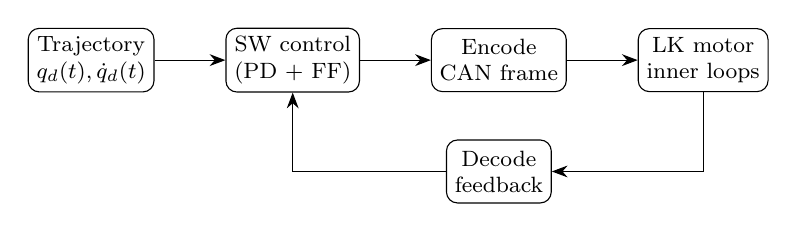
\begin{tikzpicture}[
   node distance=6mm and 9mm,
   box/.style={draw,rounded corners,align=center,font=\footnotesize,
               minimum height=8mm,inner sep=3pt},
   >={Stealth[length=2mm]}]
  \node[box] (traj) {Trajectory\\$q_d(t),\dot q_d(t)$};
  \node[box,right=of traj] (ctrl) {SW control\\(PD + FF)};
  \node[box,right=of ctrl] (enc) {Encode\\CAN frame};
  \node[box,right=of enc] (motor) {LK motor\\inner loops};
  \node[box,below=of enc] (dec) {Decode\\feedback};
  \draw[->] (traj)--(ctrl);
  \draw[->] (ctrl)--(enc);
  \draw[->] (enc)--(motor);
  \draw[->] (motor)|-(dec);
  \draw[->] (dec)-|(ctrl);
\end{tikzpicture}
\end{center}

% =====================================================================
\section{CAN Bus Communication}
% =====================================================================

\subsection{Physical and data-link layer}
CAN (Controller Area Network) is a differential, multi-drop serial bus. Here it
is accessed through Linux \textbf{SocketCAN} using the \code{python-can} library,
with a USB--CAN adapter presented as interface \code{can0}. The bus runs at
\textbf{\SI{1}{\mega\bit\per\second}}.

\begin{quote}\small
\textbf{Important:} for SocketCAN the bit rate is fixed at the \emph{link}
level, not by software:
\begin{center}\code{sudo ip link set can0 up type can bitrate 1000000}\end{center}
The \code{bitrate=1\_000\_000} keyword passed to \code{can.Bus} is ignored by
the SocketCAN backend.
\end{quote}

\subsection{Frame structure}
Every command is a standard (11-bit identifier) data frame with exactly
\textbf{8 data bytes}. For a single-motor command/reply the identifier is
\begin{equation}
  \text{arbitration\_id} = \mathtt{0x140} + \text{motor\_id}.
\end{equation}
The motor replies on the \emph{same} identifier. Byte~0 (\code{DATA[0]}) is
always the \textbf{command byte}; bytes 1--7 carry parameters or status,
laid out per command:
\[
\underbrace{\texttt{DATA[0]}}_{\text{command}}\;
\underbrace{\texttt{DATA[1]}\cdots\texttt{DATA[7]}}_{\text{7 payload bytes}}
\]

\subsection{Integer encoding: little-endian two's complement}
Multi-byte integers are transmitted \textbf{least-significant byte first}
(little-endian). Signed values use two's complement over the chosen byte width.

\paragraph{Encoding} For a value $v$ stored in $n$ bytes, the helper first maps
negatives into the unsigned range,
\begin{equation}
  \tilde v =
  \begin{cases}
    v, & v \ge 0,\\[2pt]
    v + 2^{8n}, & v < 0,
  \end{cases}
\end{equation}
then extracts byte $i$ (for $i = 0,\dots,n-1$) as
\begin{equation}
  b_i = \left\lfloor \tilde v / 2^{8i} \right\rfloor \bmod 256
       = (\,\tilde v \gg 8i\,)\;\&\;\mathtt{0xFF}.
\end{equation}

\paragraph{Decoding} Given bytes $b_0,\dots,b_{n-1}$ the magnitude is
reconstructed and the sign restored from the most-significant bit of the top
byte:
\begin{equation}
  v = \sum_{i=0}^{n-1} b_i\,2^{8i}
      \;-\;
      \begin{cases}
        2^{8n}, & b_{n-1} \ge 128 \ \text{(MSB set)},\\
        0, & \text{otherwise.}
      \end{cases}
\end{equation}
These are implemented as \code{\_decimal\_to\_byte} and
\code{\_byte\_to\_decimal} and underpin every parameter and every status field.

\subsection{Command set}
\begin{center}
\begin{tabular}{@{}llp{8.2cm}@{}}
\toprule
\textbf{Cmd} & \textbf{Method} & \textbf{Function} \\
\midrule
\texttt{0x88} & \code{motor\_run}                 & Enable / power the motor.\\
\texttt{0x81} & \code{motor\_stop}                & Stop motion, keep state.\\
\texttt{0x80} & \code{motor\_shutdown}            & Power off, clear turns/commands.\\
\texttt{0x9A} & \code{read\_motor\_status\_1}     & Temp, voltage, current, state, errors.\\
\texttt{0x9B} & \code{clear\_error\_flags}        & Clear error state.\\
\texttt{0x9C} & \code{read\_motor\_status\_2}     & Temp, $i_q$, speed, encoder.\\
\texttt{0x9D} & \code{read\_motor\_status\_3}     & Temp, phase currents $A,B,C$.\\
\texttt{0xA0} & \code{open\_loop\_control}        & Open-loop power (MS series).\\
\texttt{0xA1} & \code{torque\_loop\_control}      & Current/torque closed loop.\\
\texttt{0xA2} & \code{speed\_loop\_control}       & Velocity closed loop.\\
\texttt{0xA3/0xA4} & \code{multi\_turn\_position\_control} & Absolute multi-turn position ($\pm$ speed cap).\\
\texttt{0xA5/0xA6} & \code{single\_turn\_position\_control}& Absolute single-turn position.\\
\texttt{0xA7/0xA8} & \code{incremental\_position\_control} & Relative position step.\\
\texttt{0x90} & \code{read\_encoder\_data}        & Encoder value, raw, offset.\\
\texttt{0x92} & \code{read\_multi\_turn\_angle}   & Multi-turn angle (\SI{0.01}{\degree}/LSB).\\
\texttt{0x94} & \code{read\_single\_turn\_angle}  & Single-turn angle ($0$--$35999$).\\
\texttt{0x19} & \code{set\_zero\_position}        & Persist current pos.\ as zero (flash).\\
\texttt{0x95} & \code{set\_position\_to\_angle}   & Reassign current pos.\ (RAM).\\
\bottomrule
\end{tabular}
\end{center}

\subsection{Request--response and timing}
Each method \emph{sends} a frame and \emph{blocks} waiting for the matching
reply (\code{\_receive\_response}, default timeout \SI{0.5}{\second}, polling in
\SI{50}{\milli\second} slices). The call returns \code{None} on timeout. This
synchronous round-trip is the dominant factor limiting control-loop rate
(Section~\ref{sec:rate}).

% =====================================================================
\section{Units, Gains, and Physical Conversions}
\label{sec:gains}
% =====================================================================

The motor reports and accepts values in raw LSB units at the \emph{motor} shaft.
The robot cares about the \emph{output} shaft (after the gearbox), in degrees,
\dps{}, and newton-metres. \code{config.py} stores the conversion gains.

\subsection{Gear reduction}
The actuator has a reduction such that
\begin{equation}
  \theta_{\text{out}} = r_g\,\theta_{\text{motor}}, \qquad r_g = 0.1,
\end{equation}
i.e.\ a $10:1$ reduction (the output shaft turns one tenth of the motor shaft,
with $10\times$ the torque). This factor of $0.1$ appears inside every gain.

\subsection{Position}
The position command (\texttt{0xA4}) uses \SI{0.01}{\degree}/LSB at the motor
shaft. To move the \emph{output} by $\theta$ degrees:
\begin{equation}
  N_{\text{cmd}}
   = \underbrace{\frac{\theta}{r_g}}_{\text{motor deg}}
     \cdot \underbrace{\frac{1}{\SI{0.01}{\degree\per\lsb}}}_{=100}
   = \frac{\theta}{0.1}\cdot 100
   = \theta \cdot 1000
   \;\equiv\; \theta \cdot \texttt{pos\_gain}.
\end{equation}
Hence $\boxed{\texttt{pos\_gain} = 1000\ \text{LSB}/\si{\degree}_{\text{out}}}$.
Inversely, an output angle is recovered from a position-loop count by dividing by
\code{pos\_gain}.

\subsection{Velocity --- command and feedback}
\paragraph{Command (speed loop, \texttt{0xA2}).} Unit \SI{0.01}{\dpsu\per\lsb} at the
motor. By the same reasoning as position,
\begin{equation}
  N_{\dot\theta} = \dot\theta\cdot \frac{1}{r_g}\cdot 100
                 = \dot\theta\cdot 1000 \equiv \dot\theta\cdot\texttt{vel\_gain},
  \qquad \texttt{vel\_gain}=1000.
\end{equation}
\paragraph{Feedback (status 2).} Speed is reported at \SI{1}{\dpsu\per\lsb} at the
\emph{motor} shaft, so the output velocity is
\begin{equation}
  \dot\theta_{\text{out}} = \frac{\texttt{spd\_raw}}{\texttt{vel\_state\_gain}},
  \qquad \texttt{vel\_state\_gain} = \frac{1}{r_g}=10 .
\end{equation}

\subsection{Encoder}
A \textbf{single-turn} absolute encoder reports
$\texttt{enc}\in[0,\,65535]$ (16-bit) for one revolution of the output:
\begin{equation}
  \theta_{\text{enc}} = \texttt{enc}\cdot\texttt{encoder\_gain},
  \qquad \texttt{encoder\_gain} = \frac{360}{65535}\ \si{\degree\per\lsb}.
\end{equation}
Because it is single-turn it \emph{wraps} at \SI{360}{\degree}; multi-turn
motion must be reconstructed in software (Section~\ref{sec:unwrap}).

\subsection{Torque and current}
The motor returns the quadrature current command $i_q$ (\code{int16}). Output
torque is obtained through a single lumped calibration constant:
\begin{equation}
  \tau_{\text{out}} = \frac{\texttt{iq\_raw}}{\texttt{torque\_gain}},
  \qquad \texttt{torque\_gain} = 206.04\ \frac{\text{LSB}}{\si{\newton\meter}} .
\end{equation}
Physically this constant bundles the current LSB scale ($\tfrac{33}{4096}$ or
$\tfrac{66}{4096}$ A/LSB depending on model), the motor torque constant $K_t$,
the gear ratio $1/r_g$, and drivetrain efficiency $\eta$:
\begin{equation}
  \tau_{\text{out}} = \texttt{iq\_raw}\cdot(\text{A/LSB})\cdot K_t\cdot \frac{1}{r_g}\cdot\eta
  \;\;\Longrightarrow\;\;
  \frac{1}{\texttt{torque\_gain}} = (\text{A/LSB})\,K_t\,\frac{\eta}{r_g}.
\end{equation}

\subsection{Sign conventions}
\label{sec:signs}
Each joint has a direction multiplier $d\in\{+1,-1\}$ (\code{dir\_1},
\code{dir\_2}) chosen so that the robot's positive joint direction matches the
desired convention. It is applied symmetrically: \emph{multiply when commanding,
multiply when reading}. For a physical quantity $x$ and its raw counterpart
$x_{\text{raw}}$,
\begin{equation}
  x_{\text{cmd,raw}} = \text{gain}\cdot d\cdot x, \qquad
  x_{\text{meas}} = d\cdot \frac{x_{\text{raw}}}{\text{gain}} .
\end{equation}

\begin{center}
\begin{tabular}{@{}lll@{}}
\toprule
\textbf{Quantity} & \textbf{Gain (name)} & \textbf{Relation} \\
\midrule
Position cmd     & \code{pos\_gain}$=1000$        & $N=\theta\cdot d\cdot 1000$ \\
Velocity cmd     & \code{vel\_gain}$=1000$        & $N=\dot\theta\cdot d\cdot 1000$ \\
Velocity fb      & \code{vel\_state\_gain}$=10$   & $\dot\theta = d\cdot\texttt{spd}/10$ \\
Encoder          & \code{encoder\_gain}$=360/65535$& $\theta=d\cdot\texttt{enc}\cdot g_e$ \\
Torque           & \code{torque\_gain}$=206.04$   & $\tau = d\cdot\texttt{iq}/206.04$ \\
\bottomrule
\end{tabular}
\end{center}

% =====================================================================
\section{Worked Numerical Examples}
% =====================================================================

This section traces concrete numbers all the way to bytes, to make the encoding
and the gains tangible.

\subsection{Encoding a position command}
Goal: move the \emph{output} shaft of motor id $1$ to \SI{30}{\degree} with a
speed cap of \SI{600}{dps} (motor-shaft units), using
\code{multi\_turn\_position\_control}.

\begin{enumerate}[nosep]
  \item \textbf{Angle to LSB:} $N = 30 \times \texttt{pos\_gain} = 30\times 1000 = 30000$ LSB.
  \item \textbf{$30000$ in 4 little-endian bytes:} $30000 = \mathtt{0x7530}$, so
        bytes (low$\to$high) are $\mathtt{0x30},\mathtt{0x75},\mathtt{0x00},\mathtt{0x00}$.
  \item \textbf{Speed $600$ in 2 bytes:} $600=\mathtt{0x0258}\Rightarrow
        \mathtt{0x58},\mathtt{0x02}$.
  \item \textbf{Assemble the \texttt{0xA4} frame} ($\texttt{DATA}=[\,0,\ \text{speed}(2),\ \text{angle}(4)\,]$ with the command byte prepended):
\end{enumerate}
\begin{center}
\begin{tabular}{@{}lcccccccc@{}}
\toprule
byte & 0 & 1 & 2 & 3 & 4 & 5 & 6 & 7\\
\midrule
value & \texttt{0xA4} & \texttt{0x00} & \texttt{0x58} & \texttt{0x02} & \texttt{0x30} & \texttt{0x75} & \texttt{0x00} & \texttt{0x00}\\
role & cmd & --- & spd\textsubscript{lo} & spd\textsubscript{hi} & ang\textsubscript{0} & ang\textsubscript{1} & ang\textsubscript{2} & ang\textsubscript{3}\\
\bottomrule
\end{tabular}
\end{center}
This frame is sent on arbitration id $\mathtt{0x140}+1 = \mathtt{0x141}$.

\subsection{Negative values (two's complement)}
To command $-30000$ LSB in 4 bytes: add $2^{32}$ to get
$4294937296 = \mathtt{0xFFFF8AD0}$, giving bytes
$\mathtt{0xD0},\mathtt{0x8A},\mathtt{0xFF},\mathtt{0xFF}$. On decode, the top byte
$\mathtt{0xFF}\ge 128$ flags a negative, so $2^{32}$ is subtracted back.

\subsection{Decoding a status-2 reply}
Suppose the reply payload is
$[\mathtt{0x9C},\mathtt{0x1A},\mathtt{0x12},\mathtt{0x00},\mathtt{0x64},\mathtt{0x00},\mathtt{0x00},\mathtt{0x40}]$:
\begin{itemize}[nosep]
  \item temperature $=\mathtt{0x1A}=\SI{26}{\celsius}$;
  \item $i_q = \mathtt{0x0012}=18$ LSB $\Rightarrow \tau = 18/206.04 \approx \SI{0.087}{\newton\meter}$;
  \item speed $=\mathtt{0x0064}=100$ (motor dps) $\Rightarrow 100/10 = \SI{10}{dps}$ output;
  \item encoder $=\mathtt{0x4000}=16384 \Rightarrow 16384\times\tfrac{360}{65535}\approx\SI{90.0}{\degree}$.
\end{itemize}

\subsection{Velocity and torque commands}
\begin{itemize}[nosep]
  \item \textbf{Velocity:} \SI{60}{dps} output $\Rightarrow
        N = 60\times\texttt{vel\_gain} = 60000$ LSB ($=\mathtt{0xEA60}$).
  \item \textbf{Torque:} \SI{2}{\newton\meter} $\Rightarrow
        i_q = 2\times\texttt{torque\_gain} = 412$ LSB ($=\mathtt{0x019C}$), well
        within the $\pm2048$ range.
\end{itemize}

% =====================================================================
\section{Motor Control Modes}
% =====================================================================

The driver implements three nested closed loops on-board; the host selects which
one to command.

\subsection{Background: brushless torque and FOC}
The actuator is a three-phase brushless DC (BLDC / PMSM) motor. Its driver uses
\textbf{field-oriented control (FOC)}: the three phase currents are transformed
(Clarke + Park) into a rotating frame aligned with the rotor, giving a
\emph{direct} component $i_d$ and a \emph{quadrature} component $i_q$. Torque is
produced almost entirely by $i_q$,
\begin{equation}
  \tau \approx K_t\, i_q, \qquad i_d \approx 0,
\end{equation}
so regulating $i_q$ \emph{is} regulating torque --- which is why every higher
loop ultimately outputs an $i_q$ reference, and why \code{torque\_gain} relates
$i_q$ to output torque.

\subsection{Torque (current) loop --- \texttt{0xA1}}
Commands $i_q\in[-2048,2048]$. The driver regulates winding current via
field-oriented control (FOC) so that the measured $i_q$ tracks the command,
producing torque $\tau \approx K_t i_q$. This is the innermost loop.

\subsection{Speed loop --- \texttt{0xA2}}
Commands an output velocity (in LSB, Section~\ref{sec:gains}). Internally a
PI controller drives the \emph{torque} loop:
\begin{equation}
  i_q^{\text{ref}} = K_{p}^{v}\,(\dot\theta_{\text{ref}}-\dot\theta)
                   + K_{i}^{v}\!\int (\dot\theta_{\text{ref}}-\dot\theta)\,dt .
\end{equation}
This is the loop used by the trajectory follower.

\subsection{Position loop --- \texttt{0xA3/0xA4}}
Commands an absolute multi-turn angle, with an optional maximum-speed cap
($\texttt{0xA4}$). Internally a position controller feeds the speed loop, which
feeds the torque loop --- a full \textbf{cascade}:
\begin{center}
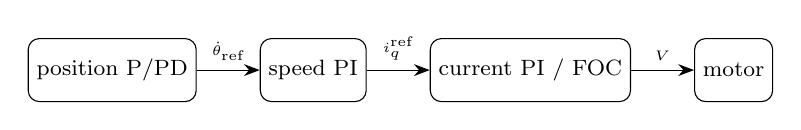
\begin{tikzpicture}[
   node distance=8mm,
   box/.style={draw,rounded corners,font=\footnotesize,minimum height=8mm,inner sep=3pt},
   >={Stealth[length=2mm]}]
  \node[box] (p) {position P/PD};
  \node[box,right=of p] (v) {speed PI};
  \node[box,right=of v] (i) {current PI / FOC};
  \node[box,right=of i] (m) {motor};
  \draw[->] (p)--node[above,font=\tiny]{$\dot\theta_{\text{ref}}$}(v);
  \draw[->] (v)--node[above,font=\tiny]{$i_q^{\text{ref}}$}(i);
  \draw[->] (i)--node[above,font=\tiny]{$V$}(m);
\end{tikzpicture}
\end{center}
The \code{max\_speed} argument bounds the inner velocity reference and is the
simplest way to make a point-to-point move slower or faster.

% =====================================================================
\section{Leg Kinematics and Dynamics}
% =====================================================================

To interpret joint commands at the foot we model the leg as a planar 2R chain:
hip angle $q_1$, knee angle $q_2$, link lengths $\ell_1$ (thigh) and $\ell_2$
(shin).

\subsection{Forward kinematics}
With angles measured from the $+x$ axis and the chain rooted at the hip, the foot
position $(x,y)$ is
\begin{align}
  x &= \ell_1\cos q_1 + \ell_2\cos(q_1+q_2),\\
  y &= \ell_1\sin q_1 + \ell_2\sin(q_1+q_2).
\end{align}

\subsection{Jacobian and static force mapping}
Differentiating, the foot velocity relates to joint rates through the Jacobian
$J(q)$:
\begin{equation}
  \begin{bmatrix}\dot x\\ \dot y\end{bmatrix}
  = J(q)\,\dot q,\qquad
  J =
  \begin{bmatrix}
   -\ell_1 s_1 - \ell_2 s_{12} & -\ell_2 s_{12}\\
    \ell_1 c_1 + \ell_2 c_{12} &  \ell_2 c_{12}
  \end{bmatrix},
\end{equation}
where $s_1=\sin q_1$, $c_{12}=\cos(q_1+q_2)$, etc. By the principle of virtual
work, a desired ground-reaction / foot force $\mathbf F$ maps to joint torques as
\begin{equation}
  \boxed{\;\boldsymbol\tau = J(q)^{\!\top}\,\mathbf F\;}
\end{equation}
This is how a force at the foot (e.g.\ supporting body weight, or a desired
push-off) is turned into the $\tau$ each joint must produce --- and hence, via
\code{torque\_gain}, into an $i_q$ command.

\subsection{Joint-space dynamics}
The leg obeys the manipulator equation
\begin{equation}
  M(q)\,\ddot q + C(q,\dot q)\,\dot q + g(q) = \boldsymbol\tau,
\end{equation}
with inertia matrix $M$, Coriolis/centrifugal term $C$, and gravity $g$. A
model-based controller would compute a feedforward
$\boldsymbol\tau_{\text{ff}} = M\ddot q_d + C\dot q_d + g$ and add a PD term;
the present software uses the motor's internal loops instead of an explicit
inverse-dynamics model (see next section).

\subsection{Cartesian (foot-space) impedance --- the next step}
The most useful capability for a leg is to control the \emph{foot} rather than
the individual joints. Define a desired foot position $\mathbf x_d$ and a virtual
spring--damper in Cartesian space:
\begin{equation}
  \mathbf F = K_x\,(\mathbf x_d - \mathbf x) + D_x\,(\dot{\mathbf x}_d - \dot{\mathbf x}),
\end{equation}
where $\mathbf x$ comes from forward kinematics and $\dot{\mathbf x}=J\dot q$.
Map that desired foot force to joint torques with the Jacobian transpose, adding
gravity compensation:
\begin{equation}
  \boxed{\;\boldsymbol\tau = J(q)^{\!\top}\,\mathbf F + g(q)\;}
\end{equation}
and send each $\tau$ through the torque loop exactly as in
\code{torque\_impedance.py}. This gives a \textbf{programmable foot stiffness}:
the leg can be soft vertically but stiff horizontally, push the ground with a
chosen force, and absorb landings. Two cautions: near a \textbf{singularity}
(leg fully extended, $\det J \to 0$) the joint torques for a given foot force
blow up; and the achievable Cartesian stiffness is again limited by the
communication bandwidth of Section~\ref{sec:rate}.

% =====================================================================
\section{A Short Control-Theory Primer}
% =====================================================================

This section gives just enough feedback-control background to read the rest.

\subsection{Feedback and the PID family}
A controller drives the \emph{error} $e = x_d - x$ (desired minus measured) to
zero. The classic PID command is
\begin{equation}
  u = \underbrace{K_P\,e}_{\text{stiffness/now}}
    + \underbrace{K_I\!\int e\,dt}_{\text{removes steady error}}
    + \underbrace{K_D\,\dot e}_{\text{damping/predict}} .
\end{equation}
\begin{itemize}[nosep]
  \item \textbf{P} reacts to the present error; larger $K_P$ = stiffer and
        faster, but too large $\to$ oscillation.
  \item \textbf{I} accumulates past error to remove steady-state offset (e.g.\
        droop under constant load); too large $\to$ overshoot / windup.
  \item \textbf{D} reacts to the rate of change; it adds damping and reduces
        overshoot, but amplifies noise.
\end{itemize}
Our joint impedance (Eq.~\eqref{eq:imp}) is a \textbf{PD} controller in disguise:
$K_P$ is the spring, $K_D$ the damper. There is no integral term --- desirable
for a compliant joint, since I-action would fight external pushes.

\subsection{Feedforward}
Feedback only acts \emph{after} an error appears. \textbf{Feedforward} (FF) adds a
command computed from the plan itself --- the desired velocity $\dot q_d$ in the
tracker, or gravity $g(q)$ in the impedance loop --- so the system tracks even
with zero error. The pattern \emph{FF + PD} (plan + correction) is used
throughout this project and is the practical core of "MIT mode."

\subsection{Cascade control}
Loops can be nested: an outer loop's output is the inner loop's setpoint
(position $\to$ speed $\to$ current). Each inner loop must be \emph{faster} than
the one outside it. The motor implements this cascade on-board; our trajectory
follower adds yet another outer position loop in software on top of the speed
loop.

\subsection{Stability, delay, and sampling}
Three effects erode stability margin and cap usable gains:
\begin{itemize}[nosep]
  \item \textbf{Loop delay:} the synchronous CAN round-trip (Section~\ref{sec:rate})
        adds phase lag; the more delay, the lower the $K_P$ you can use before
        oscillation. This is why torque control is harder here than position
        control.
  \item \textbf{Sampling:} a discrete loop at rate $f_{\text{ctrl}}$ can only act
        on dynamics well below $\sim f_{\text{ctrl}}/10$. Run as fast as the bus
        allows.
  \item \textbf{Noise:} differentiating a noisy signal (for a D term) amplifies
        it; filter velocity if you add damping from measured $\dot q$.
\end{itemize}
Practical tuning recipe: raise $K_P$ until the joint just begins to buzz, back
off $\sim30\%$, then add $K_D$ to remove residual oscillation.

% =====================================================================
\section{Trajectory-Following Control}
% =====================================================================

\subsection{Why not ``MIT mode''?}
High-performance legged actuators (e.g.\ T-Motor/CubeMars AK) accept a single
\emph{impedance} frame
\begin{equation}
  \tau = K_p\,(q_d - q) + K_d\,(\dot q_d - \dot q) + \tau_{\text{ff}},
  \label{eq:mit}
\end{equation}
evaluated on the driver at several kHz. \textbf{The LK protocol used here does
not expose this combined command} --- only the separate torque, speed, and
position loops. We therefore approximate joint impedance \emph{in software}.

\subsection{Velocity feedforward + position PD}
Rather than commanding torque, we command \emph{velocity} and let the motor's
internal speed loop realise it. The host computes
\begin{equation}
  \boxed{\;\dot\theta_{\text{cmd}} = \dot q_d + K_P\,(q_d - q_{\text{meas}})\;}
  \label{eq:law}
\end{equation}
and sends it through \code{speed\_loop\_control}. Interpretation:
\begin{itemize}[nosep]
  \item $\dot q_d$ is the \textbf{feedforward}: along the planned path the joint
        already ``knows'' how fast to move, so even with zero error it tracks.
  \item $K_P(q_d-q_{\text{meas}})$ is \textbf{proportional position feedback}: it
        corrects drift and disturbance.
\end{itemize}
This is an outer position loop whose output is a velocity reference --- it
\emph{cascades} onto the motor's speed PI loop. Comparing with
Eq.~\eqref{eq:mit}, software supplies the position-spring term while the motor's
speed loop supplies the damping/torque generation; a measured-velocity term
$-K_D\dot q$ can be added later using \code{spd\_raw} from the same reply.

\subsection{Trajectory generation}
The desired path is produced analytically so that position and its exact
derivative are both available. The default is a sinusoidal swing, phase-shifted
per joint $j$:
\begin{align}
  q_{d,j}(t)      &= q_0 + A\,\sin(\omega t + \phi_j),\\
  \dot q_{d,j}(t) &= A\,\omega\,\cos(\omega t + \phi_j),
  \qquad \omega = 2\pi f,\;\; \phi_j = j\pi .
\end{align}
Using the analytic $\dot q_d$ (not a numerical difference) keeps the feedforward
clean and noise-free. Any gait curve can replace this as long as it returns the
pair $(q_d,\dot q_d)$.

\subsection{Encoder unwrapping}
\label{sec:unwrap}
The single-turn encoder $\theta_{\text{enc}}\in[0,360)$ wraps. At control rates
the per-tick change is small, so we reconstruct a continuous angle by
accumulating wrapped differences. With $\Delta = \theta_{\text{enc}}^{(k)} -
\theta_{\text{enc}}^{(k-1)}$,
\begin{equation}
  \Delta \leftarrow
  \begin{cases}
    \Delta - 360, & \Delta > 180,\\
    \Delta + 360, & \Delta < -180,\\
    \Delta, & \text{otherwise},
  \end{cases}
  \qquad
  \theta_{\text{cont}}^{(k)} = \theta_{\text{cont}}^{(k-1)} + \Delta .
\end{equation}
The startup reading is taken as the home, so $\theta_{\text{cont}}^{(0)}=0$ and
the trajectory swings about the launch position. (Validity requires
$|\dot\theta|\,\Delta t < \SI{180}{\degree}$, easily satisfied at \SI{200}{\hertz}.)

\subsection{Discretisation and loop rate}
\label{sec:rate}
The controller runs at a fixed period $\Delta t = 1/f_{\text{ctrl}}$ (default
\SI{200}{\hertz}). Each tick, for every joint in sequence, it sends one command and
waits for the reply. With $N$ joints and round-trip time $T_{\text{rt}}$, the
achievable rate is bounded by
\begin{equation}
  f_{\text{ctrl}} \le \frac{1}{N\,T_{\text{rt}}} .
\end{equation}
Because the protocol is synchronous and joints are serviced serially, this --- not
CPU --- sets the ceiling. The loop sleeps for the remainder of $\Delta t$ after
its work; if work exceeds $\Delta t$ the effective period grows. For a full leg
or quadruped, non-blocking sends or asynchronous reads are required.

% =====================================================================
\section{Position vs.\ Torque Control}
% =====================================================================

Sections~4 and~6 commanded \emph{position} or \emph{velocity}: the host says
\emph{where} the joint should be and the motor's inner loops make it stiff. An
alternative is \textbf{torque control}: the host says \emph{how hard} the joint
should push, and stiffness becomes a software choice. This distinction is
central for legged robots.

\subsection{The trade-off}
\begin{center}
\begin{tabular}{@{}p{3.2cm}p{5cm}p{5cm}@{}}
\toprule
 & \textbf{Position / velocity control} & \textbf{Torque control} \\
\midrule
Commanded quantity & where the joint goes & how hard the joint pushes \\
Joint stiffness    & very stiff (rigid)   & soft / chosen in software \\
Ground contact / impact & poor --- shock goes to gearbox and frame & good --- joint yields and absorbs impact \\
Foot force $\boldsymbol\tau = J^\top\mathbf F$ & not directly controllable & directly controllable \\
Backdrivable       & no                   & yes \\
Ease of use        & easy (motor does the work) & hard (needs model + fast loop) \\
Typical use        & arms, free-space tracking & dynamic legged robots \\
\bottomrule
\end{tabular}
\end{center}

\noindent In one line: \emph{position control is for tracking trajectories in
free space; torque control is for interacting with the ground.} Walking,
jumping, and landing all require compliance and foot-force regulation, which only
torque control provides.

\subsection{Software joint impedance}
Because the LK protocol has no combined impedance frame (Eq.~\eqref{eq:mit}), we
evaluate the impedance law on the host and send the result through the
\emph{torque} loop (\texttt{0xA1}):
\begin{equation}
  \boxed{\;\tau = K_P\,(q_d - q) + K_D\,(\dot q_d - \dot q) + \tau_{\text{ff}}\;}
  \label{eq:imp}
\end{equation}
The joint then behaves like a \textbf{virtual spring--damper} about the desired
state: $K_P$ sets stiffness, $K_D$ sets damping, and $\tau_{\text{ff}}$ is a
feedforward (e.g.\ gravity compensation). Setting $q_d=\text{const}$,
$\dot q_d=0$ gives a pure spring that can be pushed by hand and returns
softly --- the safe way to verify the loop. Unlike the cascade of Section~4, this
runs the position/velocity feedback \emph{in software} directly on top of the
current loop, so the closed-loop stiffness is exactly $K_P$ (subject to
communication bandwidth).

\subsection{Torque-to-current conversion}
The torque loop accepts a current command $i_q\in[-2048,2048]$. Using the
calibration of Section~\ref{sec:gains} and the direction sign of
Section~\ref{sec:signs}, the commanded torque becomes
\begin{equation}
  i_q^{\text{cmd}} = \operatorname{clamp}\!\big(\,d\cdot\tau\cdot\texttt{torque\_gain},\;
  -i_q^{\max},\; +i_q^{\max}\big),
\end{equation}
where the clamp $i_q^{\max}$ is a hard safety limit (default $500$, i.e.\
$\approx 500/\texttt{torque\_gain}\approx\SI{2.4}{\newton\meter}$). Always start
with low gains and a low clamp: incorrect feedback or excessive $K_P$ can command
large forces.

\subsection{Gravity feedforward}
With a known link mass $m$, gravity $g$, and centre-of-mass distance $\ell_c$, a
single-link gravity term is
\begin{equation}
  \tau_{\text{ff}} = m\,g\,\ell_c\cos q,
\end{equation}
so the joint holds its load even with small $K_P$ (genuinely compliant
load-holding). For the multi-link leg this generalises to the $g(q)$ vector of
the dynamics equation. The code ships this as a stub returning $0$ until the
leg's parameters are supplied.

\subsection{When to use which}
\begin{itemize}[nosep]
  \item \textbf{Free-space trajectory tracking (no contact):} prefer position or
        velocity-FF + PD --- simpler and stable.
  \item \textbf{Contact-rich, dynamic motion (standing soft, force control,
        jumping/landing):} use torque/impedance control.
  \item \textbf{Hardware caveat:} torque control is far more sensitive to loop
        latency than position control. The synchronous CAN round-trip
        (Section~\ref{sec:rate}) and absence of a native impedance frame are the
        real limits here --- measure $T_{\text{rt}}$ before relying on it.
\end{itemize}

% =====================================================================
\section{Code Architecture}
% =====================================================================

\subsection{File map}
\begin{center}
\begin{tabular}{@{}ll@{}}
\toprule
\textbf{File} & \textbf{Role} \\
\midrule
\code{motor\_library.py}    & \code{LKMotor} class: CAN encode/decode, all commands. \\
\code{config.py}            & Gains, directions, test angles. \\
\code{main.py}              & Single-motor position test + CSV logging. \\
\code{demo\_motors.py}      & Sequential position demo (ids 1,2), with re-zero. \\
\code{trajectory\_follow.py}& Velocity-FF + PD trajectory tracker. \\
\code{torque\_impedance.py} & Software joint impedance via the torque loop. \\
\bottomrule
\end{tabular}
\end{center}

\subsection{The \texttt{LKMotor} class}
Construction opens the bus and zeroes the cached state:
\begin{lstlisting}
m = LKMotor(bus_interface="socketcan", bus_channel="can0",
            motor_id=1, bitrate=1_000_000)
\end{lstlisting}
Internally:
\begin{itemize}[nosep]
  \item \code{\_send\_command(cmd, data)} builds the 8-byte frame at
        \code{0x140+motor\_id} and transmits it;
  \item \code{\_receive\_response(timeout)} blocks until a reply with the
        matching id arrives (or times out $\to$ \code{None});
  \item \code{\_parse\_response\_1/2/3} decode the status payloads into the
        cached fields and return them as a tuple.
\end{itemize}

\subsection{Walkthrough: \texttt{trajectory\_follow.py}}
The control law of Eq.~\eqref{eq:law}, the unwrap of
Section~\ref{sec:unwrap}, and the sign convention of Section~\ref{sec:signs}
appear directly in the inner loop:
\begin{lstlisting}
q_des, qd_des = trajectory(t, ji)      # generated path (deg, deg/s)
q_meas = cont_deg[mid] * d             # unwrapped, sign-corrected

err = q_des - q_meas                   # position error
speed_cmd = qd_des + KP * err          # velocity FF + P  (deg/s)

res = motors[mid].speed_loop_control(  # command via inner speed loop
    IQ_LIMIT,
    int(speed_cmd * d * param.vel_gain))

_, _, _, enc = res                     # encoder feedback (single-turn)
raw = enc * param.encoder_gain         # 0..360 deg
delta = raw - prev_raw[mid]            # unwrap ...
if delta > 180:  delta -= 360
elif delta < -180: delta += 360
cont_deg[mid] += delta
prev_raw[mid] = raw
\end{lstlisting}
On exit the loop commands zero speed and releases every motor, so the leg does
not run away on \code{Ctrl-C}.

\subsection{Walkthrough: \texttt{torque\_impedance.py}}
The impedance law of Eq.~\eqref{eq:imp} and the torque-to-current conversion
appear in the inner loop; note that velocity feedback $\dot q$ is now used too:
\begin{lstlisting}
q_des, qd_des = trajectory(t, ji)      # const home (spring) or sinusoid
q_meas  = cont_deg[mid] * d            # unwrapped position
qd_now  = qd_meas[mid]                 # measured velocity (from last reply)

tau = (KP * (q_des - q_meas)           # spring
       + KD * (qd_des - qd_now)        # damper
       + gravity_feedforward(q_meas, ji))   # feedforward (stub -> 0)

iq_cmd = clamp(int(tau * param.torque_gain * d), -IQ_MAX, IQ_MAX)
res = motors[mid].torque_loop_control(iq_cmd)

_, iq_raw, spd_raw, enc = res
qd_meas[mid] = d * spd_raw / param.vel_state_gain    # update velocity
# ... encoder unwrap as before ...
\end{lstlisting}
On exit the loop sends \code{torque\_loop\_control(0)} before releasing, so the
joints go limp rather than holding force.

% =====================================================================
\section{Practical Notes, Limitations, and Tuning}
% =====================================================================

\begin{itemize}[nosep]
  \item \textbf{Gain $K_P$:} start small. Too large $\to$ buzzing / instability
        (the cascade plus communication delay reduces phase margin); too small
        $\to$ sluggish tracking.
  \item \textbf{No native impedance:} stiffness/damping at the joint are limited
        by what the speed loop and software $K_P$ provide; true variable
        impedance would need the torque loop plus the model of
        Section~5.
  \item \textbf{Single-turn absolute encoder:} multi-turn position is only known
        after software unwrapping from a known home; a power cycle loses the
        continuous count.
  \item \texttt{set\_position\_to\_angle} (\texttt{0x95}) re-zeros in RAM (no
        wear, lost on power cycle); \code{set\_zero\_position} (\texttt{0x19})
        writes flash and persists --- use sparingly.
  \item \textbf{Communication ceiling:} see Section~\ref{sec:rate}; measure the
        true loop period on hardware before trusting timing.
  \item \textbf{Lost packets:} every command may return \code{None}; the
        controllers treat this as a skipped tick.
\end{itemize}

% =====================================================================
\section{Suggested Next Steps}
% =====================================================================

A roughly ordered path from the current working code toward a controllable leg:
\begin{enumerate}[nosep]
  \item \textbf{Data logging \& plots.} Log $q_d,q,\dot q,\tau$ to CSV and plot
        tracking error vs.\ time. Tune gains from data, not feel. (No hardware
        parameters needed --- do this first.)
  \item \textbf{Gravity compensation.} Fill the $\tau_{\text{ff}}=m g \ell_c\cos q$
        stub so joints hold load with low stiffness. Needs link masses, lengths,
        and centre-of-mass positions.
  \item \textbf{Safety layer.} Joint-angle limits, a torque soft-start ramp, and
        a lost-packet watchdog that goes limp on comms loss --- before pushing
        gains or attempting dynamic motion.
  \item \textbf{Cartesian foot control.} Implement FK + Jacobian and
        $\boldsymbol\tau = J^\top\mathbf F + g(q)$ for programmable foot
        stiffness and force. Needs link lengths and a defined joint-zero
        convention. This is the headline legged-robot capability.
  \item \textbf{Measure the loop rate.} Time the CAN round-trip $T_{\text{rt}}$ on
        hardware; it determines whether high-bandwidth torque control is viable
        with this protocol.
\end{enumerate}

% =====================================================================
\appendix
\section{Symbol Reference}
\begin{center}
\begin{tabular}{@{}ll@{}}
\toprule
\textbf{Symbol} & \textbf{Meaning} \\
\midrule
$q,\dot q$              & joint angle, angular velocity (output shaft) \\
$q_d,\dot q_d$          & desired joint angle / velocity \\
$\theta_{\text{out}},\theta_{\text{motor}}$ & output- / motor-shaft angle \\
$r_g=0.1$              & gear ratio (output/motor) \\
$d=\pm1$               & joint direction multiplier \\
$i_q$                  & quadrature (torque-producing) current \\
$K_t$                  & motor torque constant \\
$K_P$                  & software position-feedback gain \\
$J(q)$                 & foot Jacobian \\
$\Delta t,\,f_{\text{ctrl}}$ & control period / rate \\
\bottomrule
\end{tabular}
\end{center}

\section{Glossary}
\begin{center}
\begin{tabular}{@{}ll@{}}
\toprule
\textbf{Term} & \textbf{Meaning} \\
\midrule
CAN          & Controller Area Network --- the serial bus protocol \\
SocketCAN    & Linux CAN networking stack \\
LSB          & least-significant bit --- the raw integer step of a quantity \\
BLDC / PMSM  & brushless DC / permanent-magnet synchronous motor \\
FOC          & field-oriented control (current control in the rotor frame) \\
$i_q,i_d$    & quadrature (torque) / direct current components \\
PD / PID     & proportional--derivative / --integral--derivative control \\
FF           & feedforward (command from the plan, not the error) \\
FK / IK      & forward / inverse kinematics \\
Jacobian     & matrix mapping joint rates to foot velocity \\
dps          & degrees per second \\
impedance    & relationship between motion and force (stiffness + damping) \\
backdrivable & able to be moved by external force \\
\bottomrule
\end{tabular}
\end{center}

\end{document}
